\documentclass[11pt,a4paper, spanish]{article}
\usepackage[T1]{fontenc}
\usepackage[utf8]{inputenc}
\usepackage[spanish]{babel}
\selectlanguage{spanish}
\usepackage{graphicx}
\usepackage{listings}

\lstset{
    language=C,
    tabsize=4,
    basicstyle=\fontsize{11}{13}\ttfamily\footnotesize,
    showspaces=false,
    showstringspaces=false,
    captionpos=b,
    breaklines=true,
    literate={á}{{\'a}}1
        {ã}{{\~a}}1
        {é}{{\'e}}1
        {ó}{{\'o}}1
        {í}{{\'i}}1
        {ñ}{{\~n}}1
        {¡}{{!`}}1
        {¿}{{?`}}1
        {ú}{{\'u}}1
        {Í}{{\'I}}1
    {Ó}{{\'O}}1
}

\usepackage{multirow}
\usepackage{float}
\usepackage[caption = false]{subfig}

\setcounter{secnumdepth}{0}

\begin{document}

%  FRONTPAGE

\begin{titlepage}
  \noindent%
  \begin{tabular}{@{}p{\textwidth}@{}}
    \vspace{0.2cm}
    \begin{center}
    \Huge{\textbf{
      Data Path
    }}
    \end{center}
    \begin{center}
      \Large{
         66:20 Organizaci\'on de Computadoras
      }
    \end{center}
    \vspace{0.2cm}\\
  \end{tabular}
  \vspace{4 cm}
  \begin{center}
    {\large
      Trabajo práctico 3
    }\\
    \vspace{0.6cm}
    {\Large
    Mauro Toscano (96890)\\
    Axel Lijdens (95772)
    }
  \end{center}
  \vfill
  \begin{center}
  Univesidad de Buenos Aires - FIUBA
  \end{center}
\end{titlepage}


\tableofcontents
\pagebreak
% Prologo

\section{Objetivos}

El objetivo de este trabajo es familiarizarse con la arquitectura de una CPU MIPS, espec\'ficamente con el datapath y la implementación de instrucciones. Para ello, se deberían agregar instrucciones a diversas configuraciones de CPU provistas por el simulador DrMIPS

\section{Alcance}

Este trabajo práctico es de elaboración grupal, evaluación individual, y de carácter obligatorio para todos alumnos del curso.

\section{Requisitos}

El trabajo deberá ser entregado personalmente, en la fecha estipulada, con una carátula que contenga los datos completos de todos los integrantes.

Además, es necesario que el trabajo práctico incluya (entre otras cosas, ver sección 8), la presentación de los resultados obtenidos, explicando, cuando corresponda, con fundamentos reales, las causas o razones de cada resultado obtenido. Por este motivo, el día de la entrega deben concurrir todos los integrantes del grupo.

El informe deber\'a respetar el modelo de referencia que se encuentra en el grupo, y se valorar\'an aquellos escritos usando la herramienta TEX / LATEX.

\section{Recursos}

Usaremos el programa DrMIPS para configurar y simular el data path de un procesador MIPS, tanto uniciclo como multiciclo.

\section{Fecha de entrega}

La última fecha de entrega y presentación ser\'a el jueves 28 de junio de 2018.

\section{Introducción}\label{informe}
El programa DrMIPS nos permite evaluar distintos diseños de datapath para procesadores
MIPS32, al darnos la posibilidad de organizarlo como queramos. Si bien sólo puede haber uno
de algunos de los componentes del DP (como el registro de PC o la unidad de control), podemos
poner sumadores, multiplexores, extensores de signo y conexiones arbitrariamente. También es
posible modificar el conjunto de instrucciones. Además de la estructura lógica del DP, DrMips
nos permite escribir programas simples y simular su ejecución en el DP, mostrando los valores
que toman las diversas entradas y salidas de cada elemento. El programa se puede conseguir en
https://bitbucket.org/brunonova/drmips/wiki/Home, o se puede descargar para Ubuntu,
ya sea desde el repositorio de Ubuntu (aunque la versión está desactualizada) o autorizando un
repositorio externo.

% Desarrollo

\section{Instrucciones a implementar}

\begin{enumerate}
  \item Implementar la instrucción \texttt{j} en el DP \texttt{pipeline.cpu}.
  \item Implementar la instrucción \texttt{jr} (Jump Register) en el DP \texttt{unicycle.cpu}.
  \item Implementar la instrucción \texttt{jr} en el DP \texttt{pipeline.cpu}. Verificar que no se produzcan hazards.
  \item Implementar la instrucción \texttt{jalr} (Jump and Link Register) en el DP \texttt{unicycle.cpu}.
  \item Implementar la instrucción \texttt{jalr} en el DP \texttt{pipeline.cpu}. Verificar que no se produzcan hazards.
\end{enumerate}


\section{Implementación}

% TODO: explicar brevemente lo que se hizo para el desarrollo de las instrucciones

\begin{figure}
\begin{center}
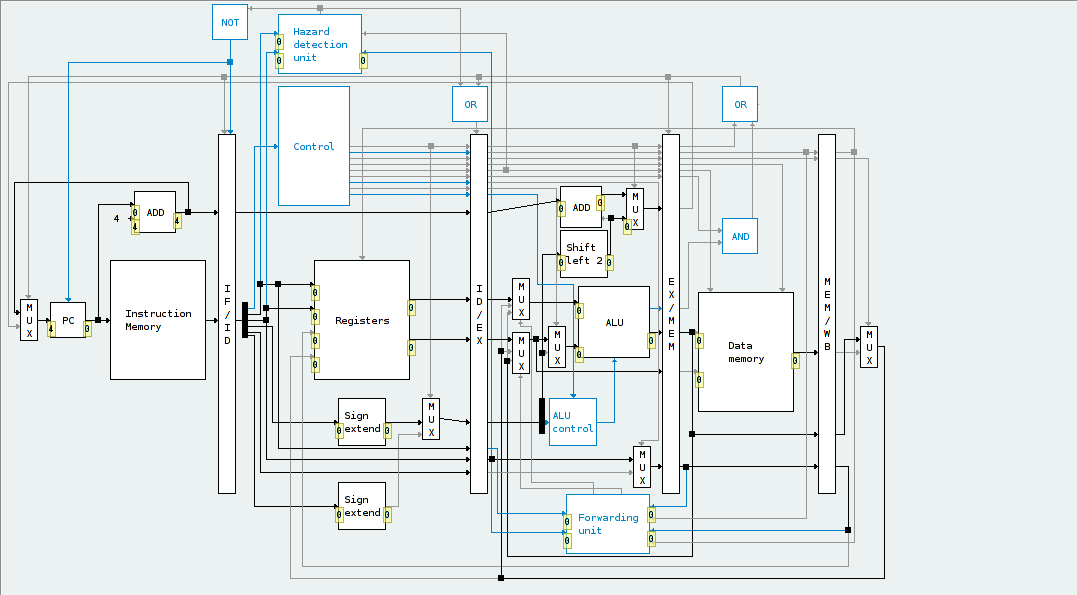
\includegraphics[width=\textwidth,height=\textheight,keepaspectratio]{img/pipeline_con_jump.png}
\caption{Pipeline con Jump}
\end{center}
\end{figure}

\begin{figure}
\begin{center}
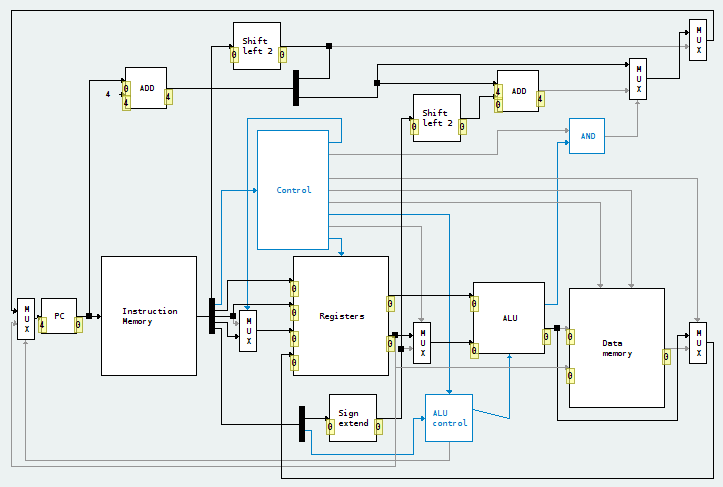
\includegraphics[width=\textwidth,height=\textheight,keepaspectratio]{img/unicycle_jr.png}
\caption{Unicycle con Jump Register}
\end{center}
\end{figure}

\begin{figure}
\begin{center}
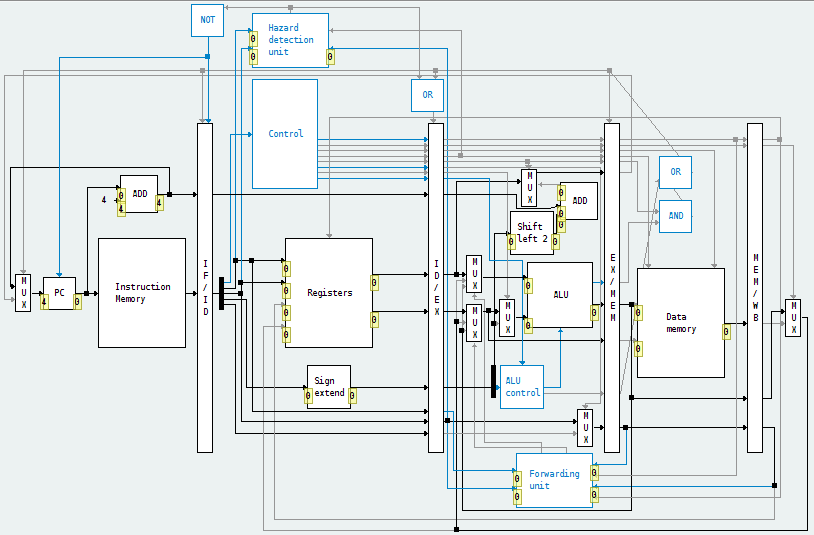
\includegraphics[width=\textwidth,height=\textheight,keepaspectratio]{img/pipeline_jr.png}
\caption{Pipeline con Jump Register}
\end{center}
\end{figure}

\begin{figure}
\begin{center}
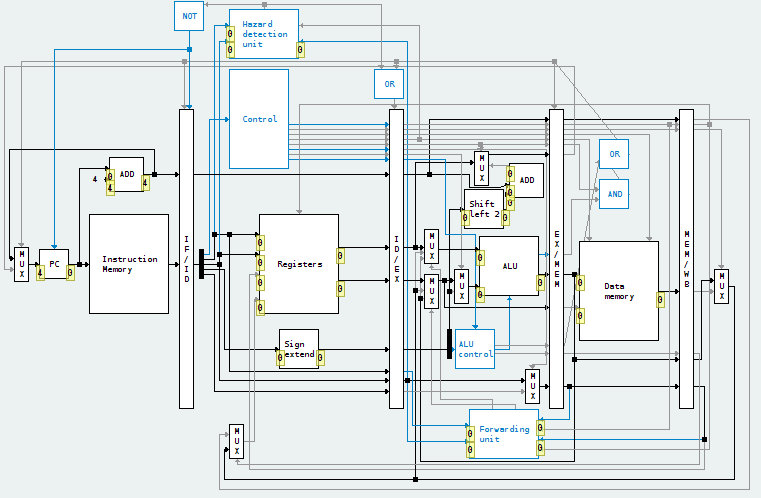
\includegraphics[width=\textwidth,height=\textheight,keepaspectratio]{img/pipeline_jalr.png}
\caption{Pipeline con Jump and Link Register}
\end{center}
\end{figure}

\begin{figure}
\begin{center}
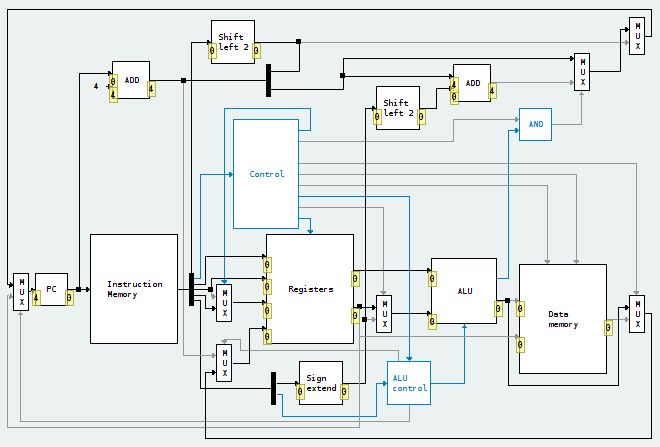
\includegraphics[width=\textwidth,height=\textheight,keepaspectratio]{img/unicycle_jalr.png}
\caption{Unicycle con Jump and Link Register}
\end{center}
\end{figure}

\section{Pruebas}

En todos los casos debe verificarse que la instrucción se ejecute correctamente. Esto implica
que el PC tome el valor deseado, y además que en el caso del DP multiciclo no se produzcan
hazards, como ser la ejecución de la instrucción siguiente al salto, o en el caso de utilizar el valor
de un registro, que éste tenga el valor correcto.


\subsection{Jump}

Para probar la instrucción \texttt{J} se utilizó el siguiente programa:

\begin{lstlisting}[numbers=left, tabsize=2, basicstyle=\fontsize{11}{13}\ttfamily, frame=single, caption={Test j}]
	li	$t0, 111
	li	$t1, 222
	j	test

	# las siguientes instrucciones no deberian ejecutarse si el salto se realiza
	li	$t0, 333
	li	$t1, 444

test:
	li $t2, 555
\end{lstlisting}

De funcionar correctamente la instrucción, el resultado debe ser \texttt{\$t0=111 , \$t1=222 y \$t2 = 555}, ya que las otras 2 instrucciones no se ejecutarían.

Se comprobo el resultado es el esperado con la implementación que lo utiliza.

\subsection{Jump Register}

Esta instrucción debe saltar a la dirección guardada en el registro indicado. El ejemplo es similar al
anterior con la diferencia que se espeficica una dirección particular.

\begin{lstlisting}[numbers=left, tabsize=2, basicstyle=\fontsize{11}{13}\ttfamily, frame=single, caption={Test jr}]
	li	$t0, 111
	li	$t1, 222
	li	$ra, 24
	jr	$ra

	# las siguientes instrucciones no deberian ejecutarse si el salto se realiza
	li	$t0, 333
	li	$t1, 444

test:
	li $t2, 555  # si las instrucciones comienzan desde la dirección 0, esta tiene la dirección 24
\end{lstlisting}

De funcionar correctamente, la ejecución debe continuar en la dirección indicada en \texttt{\$ra}, que
será la de la operación \texttt{nop} (salteando las instrucciones indicadas).

Se comprobo el resultado es el esperado con las implementaciones que lo utilizan.

\subsection{Jump and Link Register}

Eesta instrucción guarda la dirección siguiente en \texttt{\$ra} y luego realiza el salto al registro
indicado. Se utiliza el siguiente programa de prueba:

\begin{lstlisting}[numbers=left, tabsize=2, basicstyle=\fontsize{11}{13}\ttfamily, 	li	$t0, 111
	li	$t1, 222
	li	$t2, 24
	jalr	$t2, $t3

	# las siguientes 2 instrucciones no deberian ejecutarse si el salto se realiza
	addi	$t0, $t0, 333
	addi	$t1, $t1, 444

test:
       li $t2, 555
\end{lstlisting}

Al igual que el caso anterior, se debe verificar que las operaciones indicadas no se hayan ejecutado.
Además, se debe verificar que el registro \texttt{\$t3} contenga el valor correspondiente a la instrucción siguiente del \texttt{jalr}, es decir, 16.
Se comprobo el resultado es el esperado con las implementaciones que lo utilizan.

\section{Conclusiones}

DrMIPS es una herramienta útil para poder entender el funcionamiento del DP en MIPS, así
como el mecanismo de pipeline, ya que se puede ejecutar un programa paso a paso y observar los cambios
que cada instrucción realiza. Al permitir modificar libremente el DP se puede lograr un mejor
entendimiento de su funcionamiento. También es útil para simular instrucciones en 
desarrollo, ya que permite encontrar errores de la misma forma que un debugger o hace
en un lenguage de programación.

% SOlO codigos fuente hacia abajo, no hace falta editar!

\newpage

\section{Archivos .cpu}

Repositorio: https://github.com/MauroFab/orga-6620-tp3


\end{document}
\grid
\grid
